Current prediction accuracy which we achieved for the most efficient compiler flags 
is still disappointing: around 0.45\% for GCC 7.1.0.
%
We explained this in more detail in~\cite{cm:29db2248aba45e59:cd11e3a188574d80,fursin:hal-01054763}
by missing features particularly available at run-time from data sets and hardware.
%
Having a customizable experimental workflow with pluggable artifacts 
makes it relatively straightforward to analyze reactions of a given program
to the most efficient optimization across multiple data sets
and search for missing features.

First, we converted 474 different data sets from the MiDataSet suite~\cite{FCOP2007}
as pluggable CK artifacts and shared them as a zip archive (~800MB).
%
It is possible to download it from the Google Drive
from~\url{https://drive.google.com/open?id=0B-wXENVfIO82OUpZdWIzckhlRk0}
(we plan to move it to a permanent repository in the future)
and then install via CK as following:

\begin{flushleft}
\texttt{\$ ck add repo --zip=ckr-ctuning-datasets.zip --quiet}\newline
\texttt{\$ ck ls dataset --all}\newline
\texttt{\$ ck search dataset --tags=image,jpeg}\newline
\end{flushleft}

All these data sets will be immediately visible to all related programs
via the CK autotuning workflow.
%
For example, if we now run \textit{susan corners} program, CK will prompt user
a choice of 20 related images from the above data sets:

\begin{flushleft}
\texttt{\$ ck compile program:cbench-automotive-susan --speed}\newline
\texttt{\$ ck run program:cbench-automotive-susan}\newline
\end{flushleft}

   % === CK multiple datasets ==================================================================
   %CK={"action":"prepare_for_latex", "cid":"slide:82b9474cf6482c99", "file":"9f93e8520adbea97-cropped.pdf", "path":"ck-assets", "ck_image":"yes", "ck_image_width":800}
   \begin{figure*}[!htbp]
     \centering
      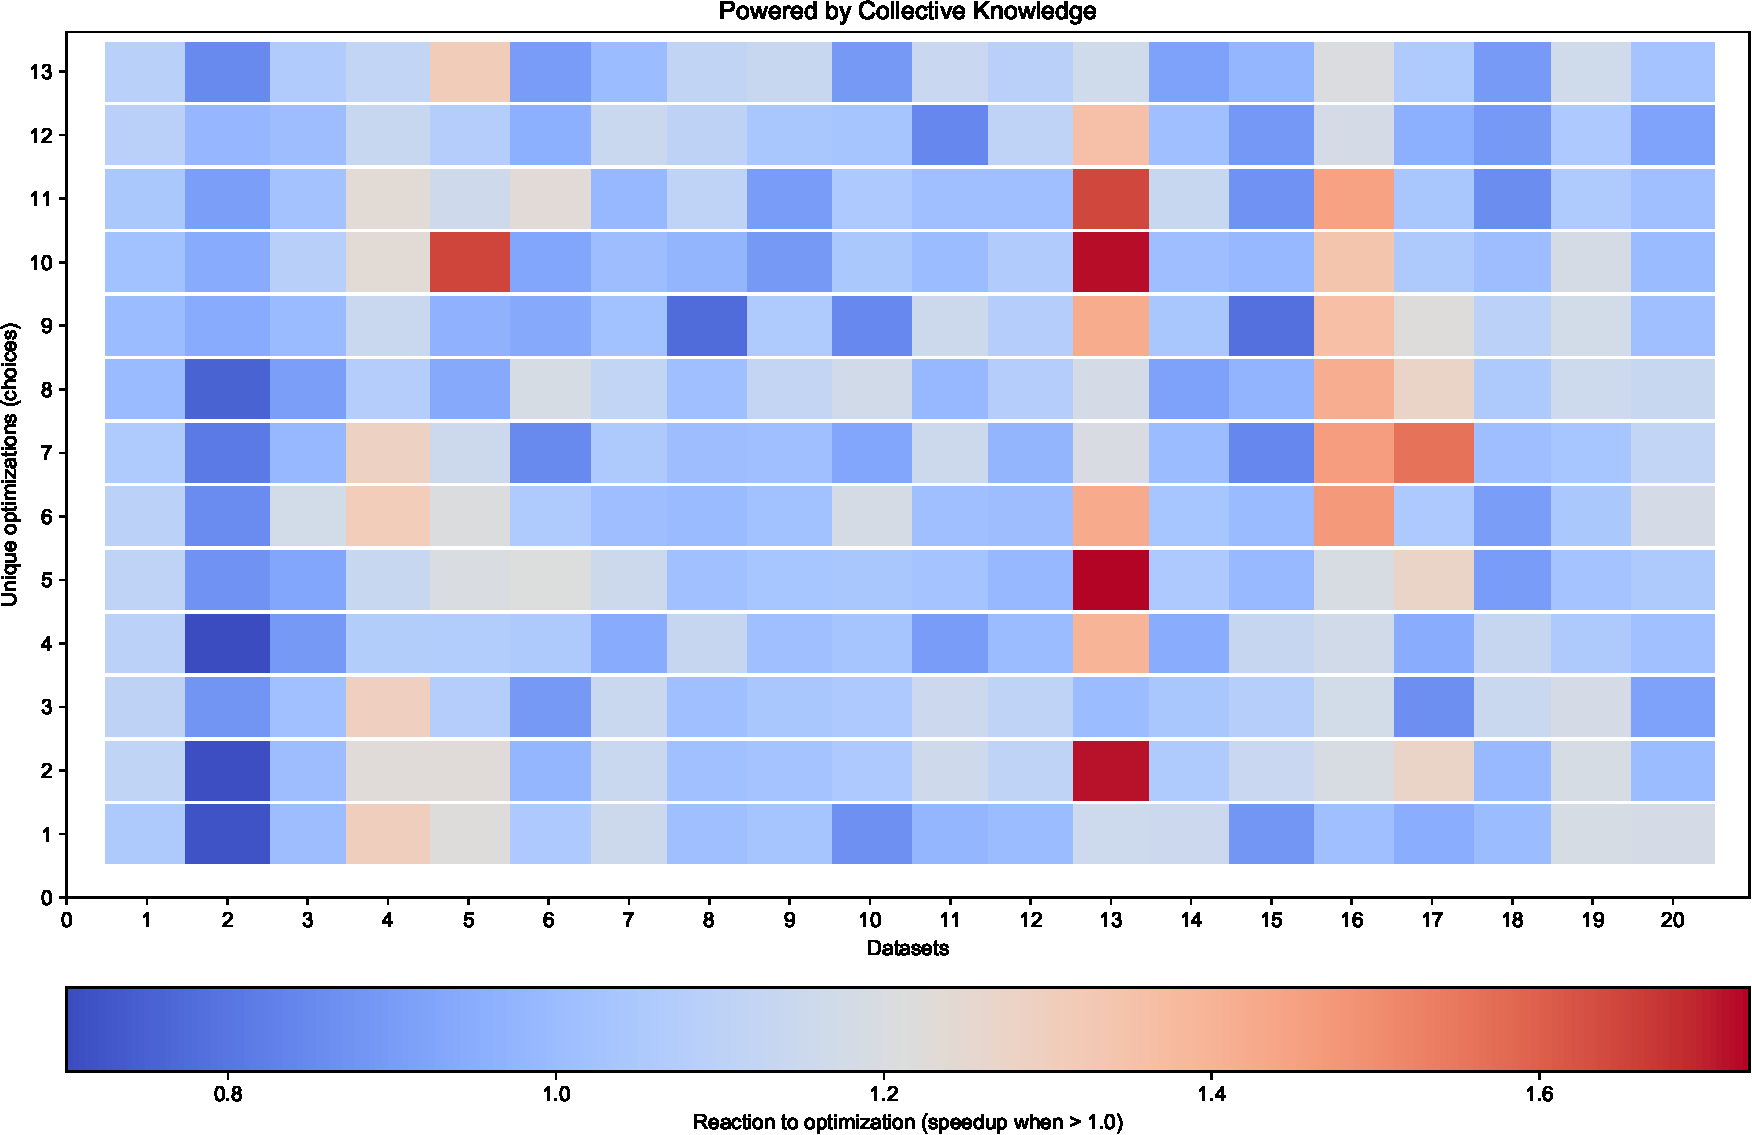
\includegraphics[width=5.8in]
      {ck-assets/9f93e8520adbea97-cropped.pdf} %CK_URL={9f93e8520adbea97-cropped.pdf}
     \caption{
       Reactions of a jpeg decoder across 20 distinct data sets (jpeg images)
       to all top performing combinations of compiler optimizations
       for GCC 7.1.0 on RPi3 device (speedups if value is more than 1.0).
     }                                         
     \label{fig:ck-datasets-jpeg-d-reactions}
   \end{figure*}

Next, we can apply all most efficient compiler optimizations 
to a given program with all data sets.
%
Figure~\ref{fig:ck-datasets-jpeg-d-reactions} shows such reactions 
(ratio of an execution time with a given optimization to an execution time 
with the default -O3 compiler optimization) of a jpeg decoder across 
20 different jpeg images from the above MiDataSet on RPi3.

One can observe that the same combination of compiler flags can both
considerably improve or degrade execution time for the same program
but across different data sets.
%
For example, data sets 4,5,13,16 and 17 can benefit from the most
efficient combination of compiler flags found by the community
with speedups ranging from 1.2 to 1.7.
%
On the other hand, it's better to run all other data sets with
the default -O3 optimization level.

Unfortunately, finding data set and other features which could easily differentiate
above optimizations is often very challenging.
%
Even deep learning may not help if a feature is not yet exposed.
%
We explain this issue in~\cite{cm:29db2248aba45e59:cd11e3a188574d80}
when optimizing real B\&W filter kernel - we managed to improve
predictions by exposing a "time of the day" feature
only via human intervention.
%
However, yet again, the CK concept is to bring the interdisciplinary
community on board to share such cases in a reproducible way 
and then collaboratively find various features to improve predictions.

Another aspect which can influence the quality of predictive models,
is that the same combinations of compiler flags are too coarse-grain
and can make different internal optimization decisions 
for different programs.
%
Therefore, we need to have an access to fine-grain optimizations
(inlining, tiling, unrolling, vectorization, prefetching, etc)
and related features to continue improving our models.
%
However, this follows our top-down optimization and modeling methodology 
which we implemented in the Collective Knowledge framework.
%
We want first to analyze, optimize and model coarse-grain behavior of shared workloads
together with the community and students while gradually adding more workloads, 
data sets, models and platforms.
%
Only when we reached the limit of prediction accuracy, 
we start gradually exposing finer-grain optimizations 
and features via extensible CK JSON interface 
while avoiding explosion in design and optimization spaces
(see details in~\cite{fursin:hal-01054763} for our previous
version of the workflow framework, Collective Mind).
%
This is much in spirit of how physicists moved from Newton's 
three coarse-grain laws of motion to fine-grain quantum mechanics.

   % === CK crowdmodeling ==================================================================
   %CK={"action":"prepare_for_latex", "cid":"slide:f8d8d41c38228c8d", "file":"37a8224467be599e-cropped.pdf", "path":"ck-assets", "ck_image":"yes", "ck_image_width":800}
   \begin{figure*}[!htbp]
     \centering
      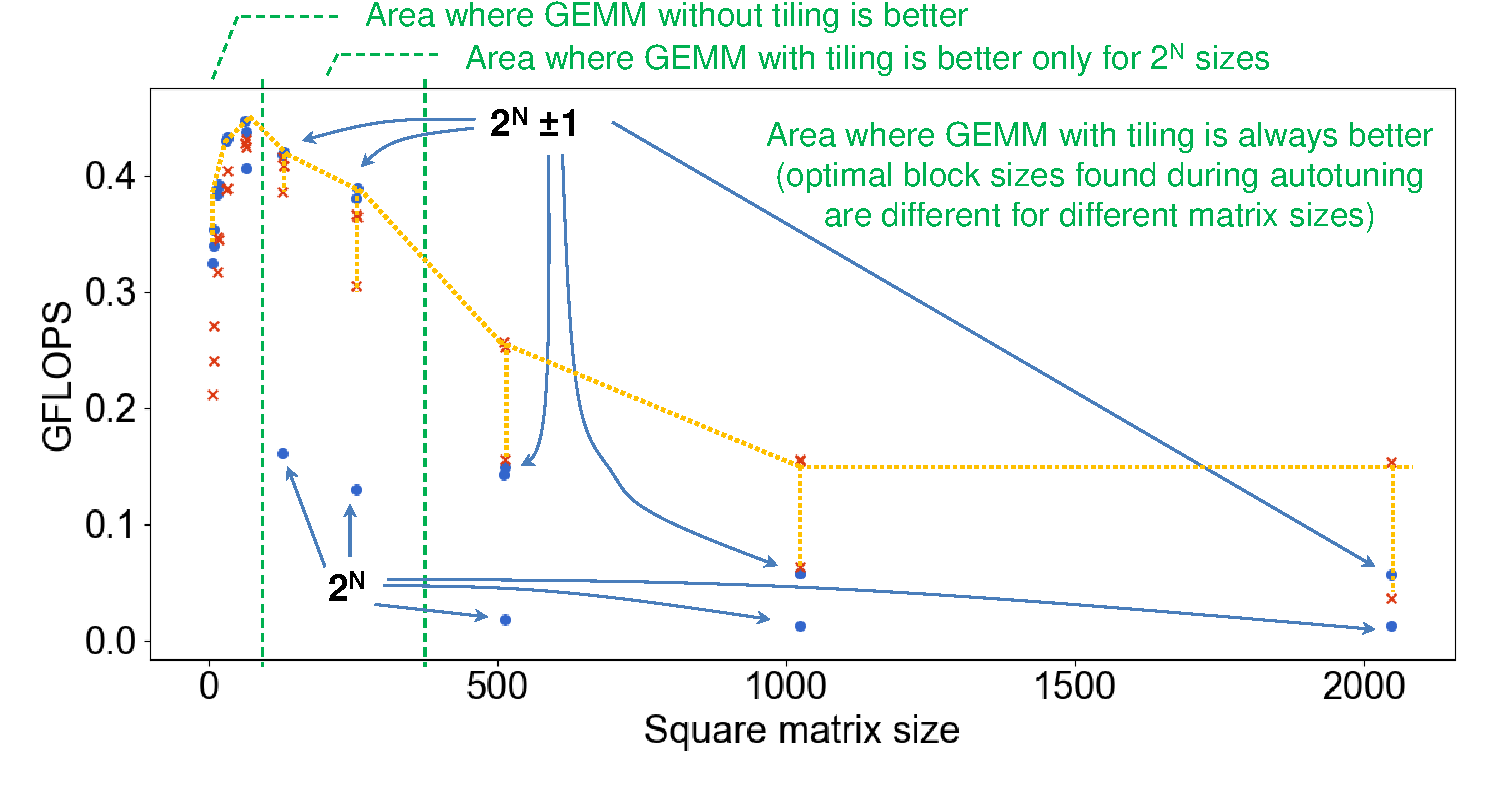
\includegraphics[width=5.5in]
      {ck-assets/37a8224467be599e-cropped.pdf} %CK_URL={37a8224467be599e-cropped.pdf}
     \caption{
      Performance of a tiled matrix multiply in GFLOPS for different square matrix sizes. 
      Blue circles show performance of original (non-blocked) matrix multiply
      while red crosses show best performance found during autotuning on RPi3 device.
     }                                         
     \label{fig:ck-datasets-input-aware-autotuning}
   \end{figure*}

To demonstrate this approach, we shared a simple skeletonized 
matrix multiply kernel from~\cite{Fur2004} in the CK format 
with blocking (tiling) parameter and data set feature 
(square matrix size) exposed via CK API:

\begin{flushleft}
\texttt{\$ ck compile program:shared-matmul-c2 --flags="-DUSE\_BLOCKED\_MATMUL=YES}\newline
\texttt{\$ ck run program:shared-matmul-c2 --env.CT\_MATRIX\_DIMENSION=128 --env.CT\_BLOCK\_SIZE=16}\newline
\end{flushleft}

We can then reuse universal autotuning (exploration) strategies
available as CK modules or implement specialized ones to explore 
exposed fine-grain optimizations versus different data sets.
%
Figure~\ref{fig:ck-datasets-input-aware-autotuning} shows matmul performance
in GFLOPS during random exploration of a blocking parameter for different square 
matrix sizes on RPi3.
%
These results are in line with multiple past studies showing that
unblocked matmul is more efficient for small matrix sizes (less than 32
on RPi3) since all data fits cache, or between 32 and 512 (on RPi3) 
if they are not power of 2.
%
In contrast, the tiled matmul is better on RPi3 for matrix sizes of power of 2 between 32 and 512,
since it can help reduce cache conflict misses, and for all matrix sizes more than 512
where tiling can help optimize access to slow main memory.

   % === CK crowdmodeling ==================================================================
   %CK={"action":"prepare_for_latex", "cid":"slide:a9de065a4bfc951d", "file":"c6d665f41a28e209-cropped.pdf", "path":"ck-assets", "ck_image":"yes", "ck_image_width":500}
   \begin{figure*}[!htbp]
     \centering
      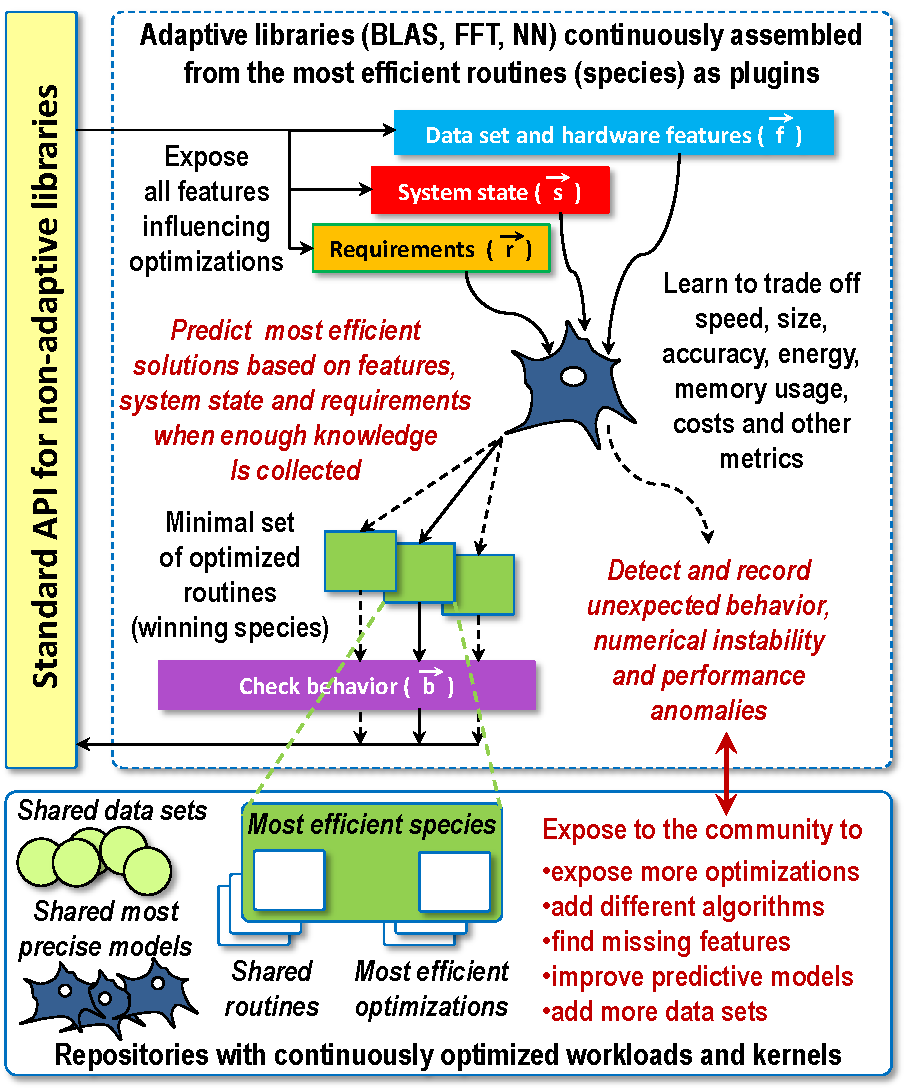
\includegraphics[width=4in]
      {ck-assets/c6d665f41a28e209-cropped.pdf} %CK_URL={c6d665f41a28e209-cropped.pdf}
     \caption{
      Enabling adaptive and self-optimizing libraries assembled from the most efficient routines
      continuously optimized by the community across different platforms and data sets. 
      These routines are selected automatically at run-time based on platform, data set and other features.
     }
     \label{fig:ck-adaptive-systems}
   \end{figure*}

Our customizable workflow can help teach students how to build efficient,
adaptive and self-optimizing libraries including BLAS, neural networks and FFT.
%
Such libraries are assembled from the most efficient routines
found during continuous crowd-tuning across numerous data sets and platforms,
and combined with fast and automatically generated decision trees  
or other more precise classifiers~\cite{DBLP:journals/ijhpca/PuschelMSXJPVJ04,5160988,LCWP2009,cm:29db2248aba45e59:cd11e3a188574d80}.
%
The most efficient routines are then selected at run-time 
depending on data set, hardware and other features as conceptually shown
in Figure~\ref{fig:ck-adaptive-systems}..

\textit{All demo scripts to generate data and graphs in this section are available in the following CK entries:}
\begin{flushleft}
\texttt{\$ ck find script:rpi3-all-autotune-multiple-datasets}\newline
\texttt{\$ ck find script:rpi3-input-aware-autotune-blas}\newline
\end{flushleft}
